\chapter{Aufgaben}
    \section{Frequenzgang der Differenzverstärkung}
Zur Untersuchung des Frequenzgangs der Differenzverstärkung $\upsilon_{\,\text{D}}$ wird an die Eingänge 1 und 2 eine Gleichtaktansteuerung $\,\text{U}_{\,\text{cm}}$ (V3) angeschlossen. Diese besitzt eine Wechselspannung von 1V. Die Wechselspannung V4 kann vernachlässigt werden, da diese auf Erde liegt. Mit dem Befehl \textbf{.ac dec 100 1 100k} wird ein Frequenzgang mit 100 Schritten zwischen 1Hz und 100kHz simuliert.
Das \textbf{dec} steht für eine Verzehnfachung der Frequenz. Der Aufbau ist in Abb.\ref{fig:schaltung} abgebildet.\\
Durch das Ausführen der Simulation, wird folgender Graph angezeigt.

 \begin{figure}[h!]
                \centering
                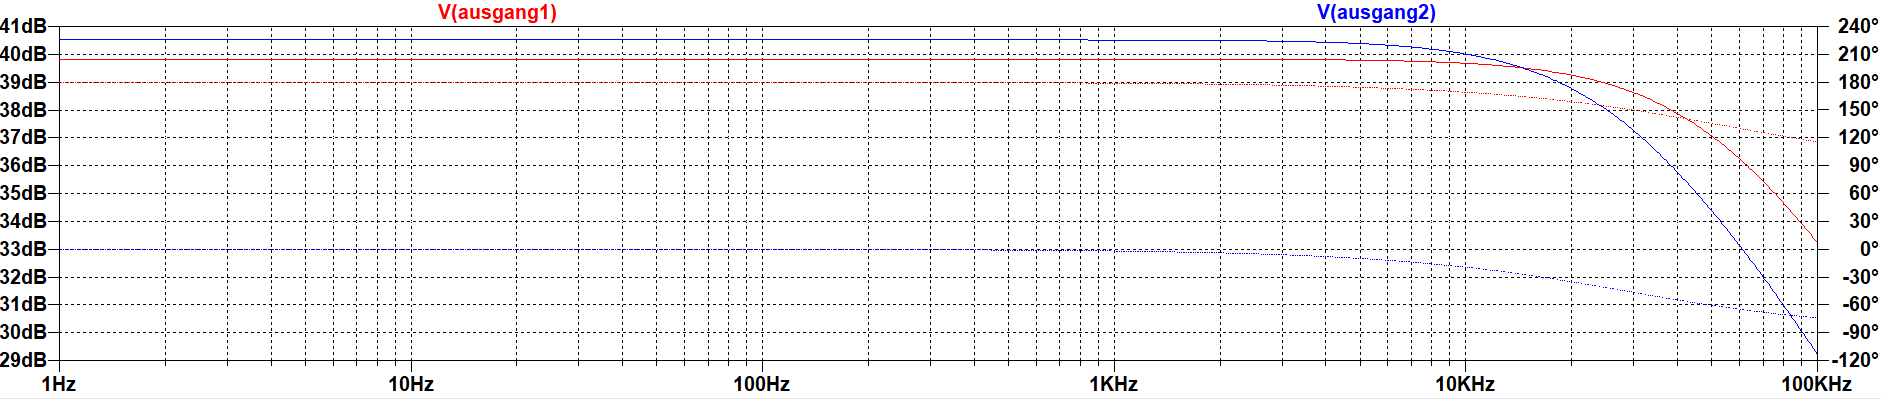
\includegraphics[width=1\linewidth]{frequenz.PNG}
                \caption{Graph des Frequenzgangs der Schaltung}
                \label{fig:frequenz}
            \end{figure}
Die obere Grenzfrequenz der Schaltung liegt im Graphen bei -3dB. Mit der Cursor-Funktion von LTSpice kann diese Frequenz für den Ausgang 1 und Ausgang 2 abgelesen werden.
  \begin{figure}[ht!]
            \begin{minipage}[c]{0.45\textwidth}
                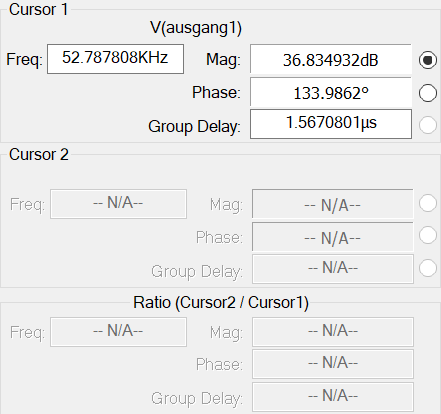
\includegraphics[width=0.9\linewidth]{cursor1.PNG}
                \caption{Anzeige der oberen Grenzfrequenz von Ausgang 1}
                \label{fig:cursor1}
            \end{minipage}
            \begin{minipage}[c]{0.45\textwidth}
                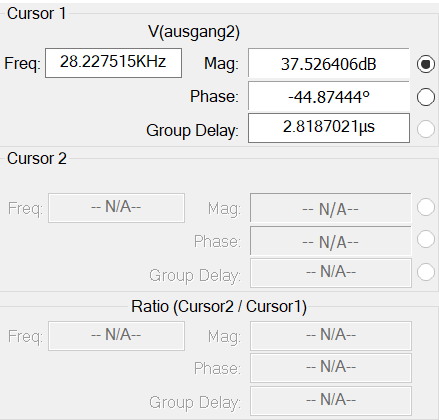
\includegraphics[width=0.9\linewidth]{cursor2.PNG}
                \caption{Anzeige der oberen Grenzfrequenz von Ausgang 2}
                \label{fig:cursor2}
            \end{minipage}
        \end{figure}
        
\newpage
Aus der Abbildung \ref{fig:frequenz} ergibt sich für den Instrumentenverstärker mit drei Operationsverstärkern eine Verstärkung $\upsilon_{\,\text{D}_{\,\text{dB}}}=39,828\,\text{dB}$ und eine obere Grenzfrequenz von $\,\text{f}_{\,\text{o}}=52,788Hz$ aus der Abbildung \ref{fig:cursor1}.\\
Aus Abbildung \ref{fig:frequenz} ist ebenfalls die Verstärkung 
$\upsilon_{\,\text{D}_{\,\text{dB}}}=40,518\,\text{dB}$ für  den Ausgang 2 des integrierten Instrumentenverstärkers zu erkennen. Die obere Grenzfrequenz des integrierten Instrumentenverstärkers ist in Abb \ref{fig:cursor2} zu finden und ergibt $\,\text{f}_{\,\text{o}}=28,227Hz$.

Beim Vergleichen der Werte von $\upsilon_{\,\text{D}_{\,\text{dB}}}$  mit den errechneten aus der Vorbereitung sind fast keine Differenzen zu erkennen.

 \begin{table}[h!]
            \centering
            \caption{Tabelle zum Vergleichen von $\upsilon_{\,\text{D}_{\,\text{dB}}}$}
            \begin{tabular}{| c | c | c |} 
            \hline
                
                & Instrumentenverstärker mit TL084 &  integrierter Instrumentenverstärker \\
                \hline\hline
              gerechnet & $\upsilon_{\,\text{D}_{\,\text{dB}}}$=39,83dB & $\upsilon_{\,\text{D}_{\,\text{dB}}}$=40,51dB  \\ 
                \hline
              simuliert & $\upsilon_{\,\text{D}_{\,\text{dB}}}$=39,828dB & $\upsilon_{\,\text{D}_{\,\text{dB}}}$=40,518dB  \\
                \hline
            \end{tabular}
            \label{tab:frequenz}
        \end{table}